%\documentclass[twoside,openright,uplatex]{jsbook} % oneside: 章ごとに改ページ.twoside: 章の初めが右側となるように改ページ.
\documentclass[oneside,openright,uplatex]{jsbook} % oneside: 章ごとに改ページ.twoside: 章の初めが右側となるように改ページ.
%\documentclass[report,uplatex]{jsbook} % oneside: 章ごとに改ページ.twoside: 章の初めが右側となるように改ページ.
%\documentclass[openany,uplatex]{jsbook} % oneside: 章ごとに改ページ.twoside: 章の初めが右側となるように改ページ.

% jsbookで余白が広すぎるのを直す
% 参照 https://oku.edu.mie-u.ac.jp/~okumura/jsclasses/
\setlength{\textwidth}{\fullwidth}
\setlength{\evensidemargin}{\oddsidemargin}

% OTF フォントを使えるようにし、複数のウェイトも使用可能にする。
% これがないと、Mac のヒラギノ環境で使われる角ゴが太すぎてみっともない。
\usepackage[deluxe]{otf}

% OT1→T1に変更し、ウムラウトなどを PDF 出力で合成文字ではなくす
\usepackage[T1]{fontenc}

% uplatex の場合に必要な処理 
\usepackage[utf8]{inputenc} % エンコーディングが UTF8 であることを明示する。
\usepackage[prefernoncjk]{pxcjkcat} % アクセントつきラテン文字を欧文扱いにする

% Helvetica と Times を sf と rm のそれぞれで使う。
% default だとバランスが悪いので、日本語に合わせて文字の大きさを調整する。
\usepackage[scaled=1.05,helvratio=0.95]{newtxtext}

\usepackage[dvipdfmx,hiresbb]{graphicx} % 画像の添付に必要
\usepackage[dvipdfmx]{color}    % 画像の添付に必要

% 表でセルを複数列で結合する
\usepackage{multicol}

% 数式の機能を拡張
\usepackage{amsmath}

% citep や citet を有効にする
\usepackage{natbib} % 参考文献を bib で管理するために必要.
\usepackage{url}    % 参考文献のリンク指定オプションに必要.

%\usepackage[hypertex]{hyperref} % url 埋め込みに必要.Usage: \href{url}{text}
%\usepackage[dvipdfmx]{hyperref}
%\hypersetup{% hyperrefオプションリスト
%  setpagesize=false,
%  bookmarksnumbered=true,%
%  bookmarksopen=true,%
%  colorlinks=true,%
%  linkcolor=blue,
%  citecolor=blue,
%}

% (Okumura, 2009) などを (Okumura 2009) とする
\setcitestyle{aysep={}}

% subfigure 環境で、(a)、(b) などの番号を左上に表示する。宇宙系の分野ではこれが一般的なはず。
\usepackage[nooneline]{subfigure}
\subfiguretopcaptrue

% 行番号を表示する。添削時のみに使い、事務提出版ではコメントアウトする
%\usepackage{lineno}
%\linenumbers

% PDF 内で外部リンクや文書内リンクを生成したい場合に使う(好みによる)
% \usepackage[dvipdfmx]{hyperref}

% newcommand を使うことで、繰り返し使う長ったらしい入力を簡単にすることができる
\makeatletter
\newcommand{\ion}[2]{#1$\;${\small\rmfamily\@Roman{#2}}\relax}%
\makeatother
\newcommand{\HI}{\mbox{\ion{H}{1}}} % 中性原子ガス(HI 領域)の例
\newcommand{\bs}{\symbol{92}} % backslash

%%%%%%%%%%%%%%%%%%%%%%%%%%%%%%%%%%%%%%%%%%%%%%%%%%%%%%%%%%%%%%%%%%%%%%%%%%%%%%%%%%%%%%%%%%%%%%%%%%%%%%%%%%%%%%%%%%%%%%%%%%%%%%

% 図を通し番号にする: http://rexpit.blog29.fc2.com/blog-entry-99.html
% \usepackage{remreset}	% removefromreset に使う
% \makeatletter
% 	\@removefromreset{figure}{chapter}
% 	\def\thefigure{\arabic{figure}}
% 
% 	\@removefromreset{table}{chapter}
% 	\def\thetable{\arabic{table}}
% 
% 	\@removefromreset{equation}{chapter}
% 	\def\theequation{\arabic{equation}}
% \makeatother

%%%%%%%%%%%%%%%%%%%%%%%%%%%%%%%%%%%%%%%%%%%%%%%%%%%%%%%%%%%%%%%%%%%%%%%%%%%%%%%%%%%%%%%%%%%%%%%%%%%%%%%%%%%%%%%%%%%%%%%%%%%%%%

\usepackage{comment} % \begin{comment} \end{comment}
\usepackage{color}   % {\bf \color{red}メモ}

\usepackage{natbib} % citep や citet を有効にする
\bibpunct[:]{[}{]}{,}{a}{}{,} % 括弧を () -> [] へ変更
%\usepackage[numbers]{natbib} % citep や citet を有効にする
%\bibpunct[:]{(}{)}{,}{a}{}{,}

\usepackage[]{multicol}         % 段組み % \begin{multicols}{2}%2段組み開始 ~ \end{multicols}%2段組み終了

\usepackage{wrapfig}            % 図の回り込みを許す.\begin{figure}~\end{figure} -> \begin{wrapfigure}{r}{90mm}~\end{wrapfigure} へ置き換え
                                % 直後の文が制御記号だと,回り込みに失敗し,文字が図下に重なるので,制御記号の直前に ''\noindent \ \ '' を挿入して回避する.

%\setlength\floatsep{0pt}         % 図と図の間の余白
%\setlength\textfloatsep{0pt}     % 本文と図の間の余白
%\setlength\intextsep{0pt}        % 本文中の図の余白
\setlength\abovecaptionskip{-3pt} % 図とキャプションの間の余白

%\usepackage{here} % \begin{figure}[H]

\renewcommand\thefootnote{\arabic{footnote})} % footnote % 脚注の調整
%\usepackage{dblfnote} % 脚注を 2 段組にする

\usepackage{threeparttable} % threeparttable % 表の下に脚注を付ける.

%%%%%%%%%%%%%%%%%%%%%%%%%%%%%%%%%%%%%%%%%%%%%%%%%%%%%%%%%%%%%%%%%%%%%%%%%%%%%%%%%%%%%%%%%%%%%%%%%%%%%%%%%%%%%%%%%%%%%%%%%%%%%%

% ソースコードの埋め込み
\usepackage{listings}
\lstset{%
  language={C},
  basicstyle={\small},%
  identifierstyle={\small},%
  commentstyle={\small\itshape},%
  keywordstyle={\small\bfseries},%
  ndkeywordstyle={\small},%
  stringstyle={\small\ttfamily},
  frame={single}, % leftline,topline,bottomline,tb OR lines, trBL,tRBl OR shadowbox, single
  breaklines=true,
  columns=[l]{fullflexible},%
  xrightmargin=0zw,%
  xleftmargin=0.5zw, % xleftmargin=3zw,%
  %numbers=left,%
  %numberstyle={\scriptsize},%
  %stepnumber=1,
  %numbersep=1zw,%
  tabsize=4, %タブの大きさ
  lineskip=-0.5ex, %行間
  linewidth=17.1cm %linewidth=16.5cm %フレームの横幅
}

%\usepackage{jlisting}
%\usepackage{listings}
%\usepackage{color}
%\definecolor{OliveGreen}{rgb}{0.0,0.6,0.0}
%\definecolor{Magenta}{cmyk}{0, 1, 0, 0}
%\definecolor{colFunc}{rgb}{1,0.07,0.54}
%\definecolor{CadetBlue}{cmyk}{0.62,0.57,0.23,0}
%\definecolor{Brown}{cmyk}{0,0.81,1,0.60}
%\definecolor{colID}{rgb}{0.63,0.44,0}
%\lstset{
%language={Matlab},                   %言語の指定
%basicstyle={\ttfamily\small},        %書体の指定
%backgroundcolor={\color[gray]{.95}}, %背景色と透過度
%keywordstyle={\color{blue}},         %キーワード(int, ifなど)の書体指定
%commentstyle={\color{OliveGreen}},   %注釈の書体 
%stringstyle=\color{Magenta},         %文字列
%frame=single,                        %枠縁(leftline,topline,bottomline,lines,trBL,shadowbox, single)
%numbers=left,                        %行番号表示
%numberstyle={\ttfamily\small},       %行番号の書体指定
%breaklines=true,                     %折り返し(自動改行)
%breakindent = 10pt,                  %自動改行後のインデント量(デフォルトでは20[pt])	
%tabsize=2,                           %タブの大きさ
%captionpos=t                         %キャプションの場所(t,b : "tb"ならば上下両方に記載)
%}
%\renewcommand{\lstlistingname}{Code} % キャプション名の指定

%%%%%%%%%%%%%%%%%%%%%%%%%%%%%%%%%%%%%%%%%%%%%%%%%%%%%%%%%%%%%%%%%%%%%%%%%%%%%%%%%%%%%%%%%%%%%%%%%%%%%%%%%%%%%%%%%%%%%%%%%%%%%%

\usepackage{packages/algorithm}
\usepackage{packages/algorithmic}

%%%%%%%%%%%%%%%%%%%%%%%%%%%%%%%%%%%%%%%%%%%%%%%%%%%%%%%%%%%%%%%%%%%%%%%%%%%%%%%%%%%%%%%%%%%%%%%%%%%%%%%%%%%%%%%%%%%%%%%%%%%%%%
% https://pureodio.hatenadiary.org/entry/20100930/1285813150

\usepackage{colortbl}
\definecolor{gray100}{gray}{1.00} % 1(白) から 0(黒)まで
\definecolor{gray090}{gray}{0.90} % 1(白) から 0(黒)まで
\definecolor{gray080}{gray}{0.80} % 1(白) から 0(黒)まで
\definecolor{gray075}{gray}{0.75} % 1(白) から 0(黒)まで
\definecolor{gray070}{gray}{0.70} % 1(白) から 0(黒)まで
\definecolor{gray060}{gray}{0.60} % 1(白) から 0(黒)まで
\definecolor{gray050}{gray}{0.50} % 1(白) から 0(黒)まで
\definecolor{gray040}{gray}{0.40} % 1(白) から 0(黒)まで
\definecolor{gray030}{gray}{0.30} % 1(白) から 0(黒)まで
\definecolor{gray020}{gray}{0.20} % 1(白) から 0(黒)まで
\definecolor{gray010}{gray}{0.10} % 1(白) から 0(黒)まで
\definecolor{gray000}{gray}{0.00} % 1(白) から 0(黒)まで


%%%%%%%%%%%%%%%%%%%%%%%%%%%%%%%%%%%%%%%%%%%%%%%%%%%%%%%%%%%%%%%%%%%%%%%%%%%%%%%%%%%%%%%%%%%%%%%%%%%%%%%%%%%%%%%%%%%%%%%%%%%%%%

\begin{document}

\begin{titlepage}


\vspace*{120truept}
\begin{center}
  \huge{学 \ 士 \ 論 \ 文 / \ 修 \ 士 \ 論 \ 文}\\
  \vspace{30truept}
%\textbf{
  \huge{タイトルが\\長い場合はいい感じに改行}\\ % title
%  \LARGE{------サブタイトル------}\\ % サブタイトル(なければコメントアウト)
%}
\vspace{100truept}
\LARGE{xx大学大学院xxxx研究科}\\
\LARGE{xxxx専攻xxxx分野xx研究室}\\
\LARGE{苗字 名前}\\
\end{center}


\end{titlepage}
 % 表紙
\thispagestyle{empty} % ページ番号を表示しない.

% レイアウトを他の章のはじめのページと揃える.
 \\
\\
\\
\\
\noindent{\Huge \sf 要旨}\\
\\
\\
\\

ハッシュテーブルは,
ハッシュ化された入力 key を配列サイズで除算した際の余り (modulo) を配列のインデックスとして値を格納することで,
key に対応する値を,定数時間で高速に取得するアルゴリズムである\footnote{コンピュータがアドレスから要素を定数時間で参照できる特性を利用している.}.
ハッシュテーブルは, key と対応した値を保持する表であることから,配列のことをテーブルと表現する.
また, key と値の対応を key-value ペアと表現する.

一般に,
ハッシュ値の剰余は配列全体に均一に分布することが望ましいが,
実際には配列の利用率を示す load factor \footnote{別名:座席利用率.} の増加に伴い衝突する.
%衝突確率を下げるには,より広い値空間に移せばよく,この操作をリハッシュと呼ぶ
%\footnote{リハッシュを行う際は,リハッシュ時間を定数時間に収めるため,通常は倍サイズの配列長に遷移させる.
%ただし,ここでの定数時間とは,繰り返し遷移させた場合のコストを1要素ごとで分割したコストが,単に O(n) となることを意味する.}
%.一般に,Chain 法.
剰余の衝突は,key-value ペアをより広い配列へ移すことで解決できる.
この操作をリハッシュと呼ぶ.
しかし,メモリ効率上,実用的な load factor を達成するためには,
リハッシュ以外の方法で衝突を解決する必要がある.

剰余衝突の解決策は,主に2種類に大別される.
1つ目は,
Chaining に代表される Open hashing\footnote{別名:Closed addressing.} である.
衝突が発生した際,新しくメモリ領域を確保し,片方向リスト\footnote{別名:linked list または singly linked list,} により現在の要素に追加する.
この手法は,
要素の削除と追加を繰り返す場合でも安定して動作するが,要素をポインタにより接続するため,
アドレス空間が連続とならず CPU キャッシュが効き難い欠点がある.
2つ目は,
Linear probing や Quadratic probing に代表される Closed hashing\footnote{別名:Open addressing.} である.
衝突が発生した際,それぞれの probing 規則に従い,隣接する空き要素に値を格納する.
Linear probing は,隣接する $1, 2, 3, ... k$ 番目の要素を線形探査する.
% 隣接する要素に値が格納されている場合は,高速に取り出せる.しかし,
配列が隙間なく埋まった場合は,
境界が分からず探査時間は大きく増加する.これを Primary clustering と呼ぶ.
% \footnote{Primary clustering と呼ぶ}.
% \href{https://en.wikipedia.org/wiki/Primary_clustering}{Primary clustering - wikipedia - 2019.06.22}}
% https://books.google.co.jp/books?id=HJ9gds_zhVEC&pg=PA186&redir_esc=y#v=onepage&q&f=false, ISBN 9780763725624 - Google Books
Quadratic probing は,隣接する $1^2, 2^2, 3^2, ... k^2$ 番目の要素を探査する.
飛び値を取るため,比較的 Primary clustering し難い.
いずれの probing も,空の要素が探査終了条件 \footnote{最悪計算量を保証するため,ホップ数を制限することもある.} の一つであるため,
要素を削除すると「要素が削除された」のか「要素が存在しない」のか判断できない.
このため,要素削除時は,削除フラグを付与する.
これらの手法は,
要素の削除と追加を繰り返す場合において,性能低下とそれに伴うリハッシュを必要とするが,
要素を隣接する要素に格納するため,CPU キャッシュが効き易い利点がある.

課題とする特性は次の通りである.
要素を挿入する際,
Open hashing は,必ず剰余値が探査すべき片方向リストの先頭アドレスを示すのに対して,
Closed hashing が示す剰余値のアドレスは probing すべき最初の要素の場合と,
挿入先の配列が使用中のため,隣接する未使用の配列に移動された要素の場合がある.
一方で,Closed hashing は Open hashing と比較してキャッシュミスを起こしにくい
\footnote{キャッシュの有効性は,全ての要素を探査する必要のある unsuccessful lookup において,特に顕著となる.
また,剰余の衝突の程度により変化する.}.
また,load factor の観点において,
Open hashing は,剰余がすべての配列番号に分布しない限り配列を使い切ることができないため,
load factor を上げるには,剰余の衝突による lookup 速度の低下を許容する必要がある.
これは,load factor と  lookup 速度がトレードオフの関係にあることを示す.
Closed hashing においても,load factor が上がるほど,配列の隙間がなくなり lookup 速度が低下する.
ただし,Quadratic probing においては特に,この速度低下は緩やかである.
\footnote{たとえば,Google は,Knuth が 80 \% 程度でリハッシュするのがよいとしている{\bf \color{red}(要出典)}とした上で,
速度を求めて google::dense\_hash\_map の load factor を 50 \% に制限している (dense\_hash\_map のコメントより).}

本研究では,既存のハッシュテーブルより lookup 速度の高い Closed hashing 手法を提案する.
まず,Closed hashing 特有の,対象となる key の剰余値自体は衝突していないにも関わらず,
これまでに衝突した隣接要素の格納先として,既に占有されている問題を解決する.
これには,
が必要となる.
そのため,た.

まず,Closed hashing の剰余値が示すアドレスに,
本来格納すべきでない隣接要素の値が格納されている場合,
必ず探査すべき要素であるように要素を入れ替える.



要素の交換には,が必要
するため,

を避けるため,Closed hashing による.

本研究では,キャッシュミスを避けるため,Closed hashing による.








\frontmatter     % make page number roman
\tableofcontents % 目次
%\listoffigures  % 図目次
%\listoftables   % 表目次

\mainmatter      % make page number arabic
\chapter{序論}
\label{chap_Introduction}

ハッシュテーブルの挙動を理解する上で,
数理モデルの示す理論的な計算量は大きな助けとなる.
図\ref{fig_taocp_v3_fig44}に\citep{knuth1998}よる比較を示す.
L は Linear probing,
U は Quadratic probing \footnote{$M \rightarrow \infty$ において,Quadratic probing と Double hashing は Uniform hashing と等価.},
S は Separate chaining の結果を示す.
図\ref{fig_taocp_v3_fig44}から分かるように,
Load factor が高くなるに従い,
平均 probe 数は上昇する傾向が見られ,
特に Linear probing では顕著である.
Quadratic probing では,
幾らか改善されるが,
いずれも
Unsuccessful lookup においては $\alpha = 0.65$ 前後,
Successful lookup においても $\alpha = 0.85$ 前後において,
急激に平均 probe 数が増加する.
この特性は,ハッシュテーブルの Load factor が閾値を超えると,
著しく性能が悪化することを意味する.
したがって,性能が悪化する手前で Load factor を制限する必要がある.
一方で,chaining を利用する C, S, SO については,
性能悪化は限られることが分かる.
このとき,
C は Coalesced Chaining\footnote{Closed hashing の一種で singly linked list により,次に辿る要素を示す.},
S は Separate chaining,
SO は Separate chaining with ordered lists である.

% Coalesced Chaining
% https://www.youtube.com/watch?v=9SPhD49ePXg
% -> singly linked list (Robin Hood の逆向きの chain.)

% taocp-v3 page.679
% As remarked above, extensive tests show that Algorithm D with two independent
% hash functions behaves essentially like uniform probing, for all practical
% purposes. In fact, double hashing is asymptotically equivalent to uniformprobing, in the limit as M → ∞ (see exercise 70).

% NOTE:   Quadratic Probing and Double Hashing have identical performance.
% Ref: 
%   page. 11
%   DatStr_152_HashTables.pdf - https://www.eecs.yorku.ca/course_archive/2003-04/F/2011/2011A/DatStr_152_HashTables.pdf

\begin{figure} % 特に強い理由がない限り、[htbp]のような指定はしないでください。
  \centering
  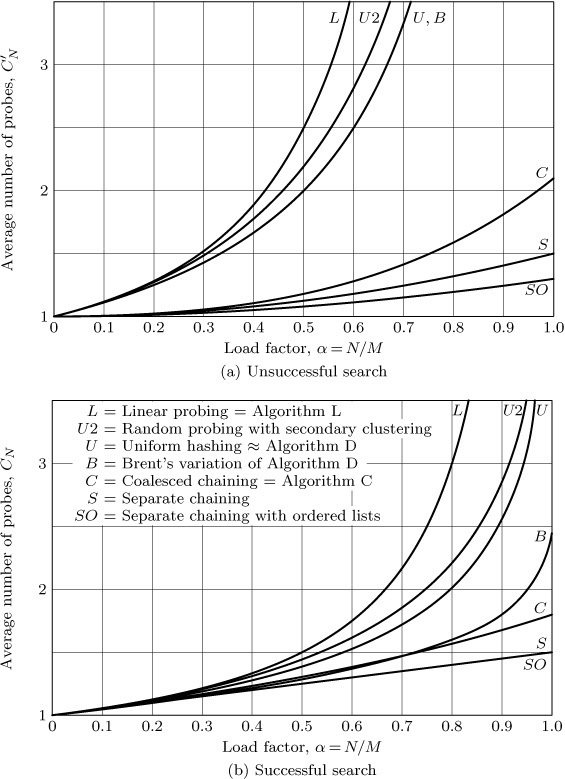
\includegraphics[width=10cm]{./figs/taocp_v3_fig44.png}
  \caption{
    Comparison of collision resolution methods: limiting values of the average number of probes as $M \rightarrow \infty$ \citep{knuth1998}.
    N は要素数,M はテーブルサイズを表す.
  }
  \label{fig_taocp_v3_fig44}
\end{figure}

%先行研究\footnote{脚注はこのように挿入します.}.

\section{先行研究}
現実的なハッシュテーブルを検討するには,
単にアルゴリズムのみならず,
対応する実実装との比較が望ましい.
ここでは,
実際に利用されているハッシュテーブルの実実装を示す.
\leavevmode \newline

{\bf std::unorderd\_map}
\samepage \\ \indent
C++ 標準のハッシュテーブル.
メモリ効率を重視しており速度は遅い.
Load factor は,しばしば 100 \% を超過する.

{\bf google::dense\_hash\_map}
\samepage \\ \indent
探査が最も高速な実装の内の 1 つで,\cite{sparsehash2005}に含まれる.
スループットで 250 query/$\mu$s 程度
\footnote{AMD Ryzen7 1700 (8C/16T) 3.7 GHz の場合.詳細は,第\ref{chap_Results}章を参照.}
の探査速度を持つことから,
探査 1 回の実行時間は 4 ns
\footnote{
  $
    250{\rm [query \slash \mu s]}
    = \frac{1}{250} {\rm [\mu s \slash query]}
    = \frac{10^3}{250} {\rm [ns \slash query]}
    = 4 {\rm [ns \slash query]}
  $
}
である.このとき,3.7 GHz の CPU では単位 clock あたりの実行時間が,
$2.7 \times 10^{-1}$ [ns/clock]
\footnote{
  $
    \frac{1}{3.7 {\rm [GHz]}}
    = \frac{1}{3.7 \times 10^9}{\rm [sec]}
    = 2.7 \times 10^{-10}{\rm [sec]}
    = 2.7 \times 10^{-1}{\rm [ns/clock]}
  $
}
であるから,1 回の探査で消費する CPU cycle は
15 clock 程度
\footnote{
  $
    \frac{ 4 {\rm [ns/query]} }{ 2.7 \times 10^{-1} {\rm [ns/clock]} }
    = \frac{ 4 }{ 2.7 \times 10^{-1} } {\rm [clock/query]}
    \simeq 15 {\rm [clock/query]}
  $
}
である.

いくつかのハッシュテーブルでは,
key のハッシュ値をテーブルサイズに丸めるために剰余演算を用いる.
整数除算に必要な CPU cycle は 14--46 clocks 程度
\footnote{
  \cite{AgnerFog2018}より AMD Ryzen7 1700 の場合.
}
であるから,dense\_hash\_map の実行時間に対して計算量が大きい.
実際に,
dense\_hash\_map では,整数除算をしておらず,
ハッシュ値の LSB \footnote{Least Significant Bit の略記.最下位ビットのこと.} から
テーブルサイズ分の bit 数だけ bit mask 演算により取り出している.
これを実現するため,テーブルサイズは常に 2 のべき乗となるように制御されている.

また,メモリ使用量を削減するため,空マークを登録する必要があり,key として使用できない.
削除マークについても同様で,key とメモリを共有しているため,削除が必要な場合は,削除マークを登録する必要があり,key として使用できなくなる.

{\bf ska::flat\_hash\_map}
\samepage \\ \indent
Robin Hood hashing の実実装の内の一つ.
条件次第で dense\_hash\_map より探査が高速であることを謳う.
Robin Hood hashing は衝突解決法の一つで,
singly linked list により,ハッシュ値の示すテーブルアドレスを示す.
本来の挿入位置が分かるため,
より近い位置に要素が移動するように調整できる.
Coalesced Chaining とは singly linked list の使い方が逆である.
実際の探査時は,Linear probing により要素を検索する.
Linear probing のコストに配慮し,
探査を $log_2(n)$ に制限している (ただし $n$ はテーブルサイズ) \cite{Skarupke2017}.

これらの特徴をまとめると,表\ref{table_hashT_cmp}のようになる.

\begin{table}[hbtp]
  \begin{center}
    \fontsize{9pt}{10pt}\selectfont
    \caption{各実装の比較.}
    \begin{tabular}{ccccccc} \hline
      \begin{tabular}{c}Implementation of\\hash table\end{tabular} & Algorism & Insert & \begin{tabular}{c}Successful\\lookup\end{tabular} & \begin{tabular}{c}Unsuccessful\\lookup\end{tabular} & Erase & \begin{tabular}{c}Memory\\efficiency\end{tabular} \rule[0pt]{0pt}{15pt} \\ \hline
      std::unorderd\_map           & Open hashing $^{a)}$   & bad   & bad  & bad  & bad   & good   \\ 
      google::dense\_hash\_map     & Closed hashing $^{b)}$ & good  & good & good & good  & medium \\
      ska::flat\_hash\_map         & Closed hashing $^{c)}$ & good  & good & good & good  & bad    \\ \hline
    \end{tabular}
    \\ 
    $^{a)}$ Chaining, 
    $^{b)}$ Quadratic probing,
    $^{c)}$ Robin Hood hashing (One of the linear probing)
    \label{table_hashT_cmp}
  \end{center}
\end{table}


\section{研究目的}

ハッシュテーブルにおいて,
単に高い探査性能を求めるだけであれば,
図\ref{fig_taocp_v3_fig44}が示すように Load factor を下げてしまえば,
どの手法も同じような性能に落ち着く.
実際に,この味付けが異なるため,
ハッシュテーブルの性能を比較する際には,
どのハッシュテーブルがどれだけのメモリを消費しているかを考慮しなくてはならず,
厳密にな比較は困難である.

しかし,現実の問題を考えるとき,
メモリ資源は有限であり,
また,高いメモリ効率を達成すれば,それだけキャッシュに乗り易くなる.
加えて,高い Load factor を達成することは,
Rehashing の発生し難い設計であることを意味し,
実利用時の安全マージンが広いことを示す.


















\chapter{アルゴリズム}
\label{chap_Algorism}

Linear probing や quadratic probing など
従来の closed hashing では,
ハッシュ先が重複していない場合でも,
別のキーの退避先として配列要素が使用中の場合,
本来 1 回目の探査でアクセスできるキーであっても,
probing により衝突を解決しなければならない.
Robin Hood hashing は,1 回でアクセスできる位置に要素を移動できるものの,
ハッシュ先の重複 \footnote{secondary clustering.} に対しては線形探査が必要となる.

本研究では,
ハッシュ先が別のキーの退避先として利用されてしまう primary clustering に付随した問題に対して,
逆方向リストを辿ることで,要素が使用済みの場合でも適切に移動し,
ハッシュ先が必ず 1 つ目の要素となるように調整する.
また,平均探査回数を削減するため,
順方向リストにより,次に探査すべき配列インデックスを示す.
メモリ使用量を削減するため,リストは int 型により相対位置を記録し,
これら順方向と逆方向を合わせて双方向リスト構造とする.
以上のアルゴリズムを実現したハッシュテーブルを,
In-place chained hash table と呼ぶこととし,
以降,省略して IpCHashT と表記する.

IpCHashT のデータ構造における提案は,本質的に \cite{ADMIS2017} の提案と同様である.
以下,
図\ref{fig_IpCHashT_struct},
図\ref{fig_IpCHashT_insert_hard_case01}〜\ref{fig_IpCHashT_insert_hard_case11},
図\ref{fig_IpCHashT_deletion_case01}〜\ref{fig_IpCHashT_deletion_case06}は,
\cite{ADMIS2017} に由来する図である.
ただし,本研究では,
挿入アルゴリズムに新しく soft insertion を採用している.
探査においても,
successful search を優先するオプションと,
unsuccessful search を優先するオプションについて新たに実装と評価を行う.
また,パディングサイズは従来固定であったが,
テーブルサイズによってパディングサイズを動的に変更することで,
テーブルサイズが小さい場合に最大 load factor が低下する問題に対処する.
加えて,テンプレートを用いて実装するにあたり,
ソフトウェアをフルスクラッチで書き直す.
要素の挿入においては,操作手順を再検討し,より簡潔な実装とする.

IpCHashT では,図\ref{fig_IpCHashT_struct}に示すデータ構造を備える.
各要素には key-value ペアの他に,linked list のための prev 要素と next 要素を持つ.
T\_shift には uint8 または uint16 型を用い,相対位置による双方向リストを構成する.
これは,ポインタ接続におけるメモリ消費量が無視できないためである
\footnote{
  例えば 64 bits CPU の場合,ポインタサイズは 64 bits であるから,T\_key と T\_val が uint64 型の場合,
  テープルサイズの 50\% が双方向リストに由来する.
}.
\leavevmode \newline

\begin{figure} % 特に強い理由がない限り、[htbp]のような指定はしないでください。
\begin{lstlisting}[language=C++]
template <class T_key, class T_val, typename T_shift>
struct element{
	element(){
		T_shift maxShift = (T_shift) 0; maxShift =~ maxShift;
		prev = maxShift;
		next = (T_shift) 0;
	}
	~element(){}
	
	T_key key;
	T_val val;
	T_shift prev;
	T_shift next;
};
\end{lstlisting}
\caption{
  IpCHashT 要素の C++ 擬似構造体.T\_key はキーの型,T\_val は val の型である.
  T\_shift は双方向リストに用いる型で,uint8 または uint16 を指定する.
  uint16 より大きな型を指定するメリットは殆どない.
  prev は 前の要素までの相対距離を,next は 次の要素までの相対距離を表す.
  ポインタにおけるアドレスとは異なり,区間 [0, max(T\_shift) - 1] の範囲でリンクを表現する.
  ただし,max(T\_shift) は T\_shift 型の取り得る最大値である.
  0 のときに自分自身を示し,max(T\_shift) - 1 がリンクできる最大距離である.区間外へのリンクはできない.
  max(T\_shift) は,予約されており,'prev==max(T\_shift)' のとき,要素が空であることを示す.
  また,'prev==0' であれば linked list の先頭であること,'next==0' であれば linked list の末尾であることがわかる.
}
\label{fig_IpCHashT_struct}
\end{figure}

\begin{figure}
  \includegraphics[scale=0.73]{./fig_algo/algorism_crop_01.pdf}
  \caption{
    図\ref{fig_IpCHashT_apparence}〜\ref{fig_IpCHashT_deletion_case06}に用いる記号.
    ``Ope.''は,実行順序を表し,``Ope. 0'' の場合は初期状態を意味する.
    下向き矢印は,ハッシュ値の示す配列アドレス上に置かれる.
    各要素は,丸 1 つと prev locator 1 つ,next locator 1 つで構成されるが,
    接続が無い場合 locator は省略される.
    点線で書かれた丸は空の要素を表し,緑の枠線と矢印は要素の移動を表す.
    バツ印は linked list の削除表す.
    配色は,青色を初期状態,赤色を要素の挿入・削除動作,緑色を要素の移動,と分かれている.
  }
  \label{fig_IpCHashT_fig_description}
%\end{figure}

%\begin{figure}
  \includegraphics[scale=0.73]{./fig_algo/algorism_crop_03.pdf}
  \caption{
    IpCHashT に挿入された要素の抽象表現.
    この場合,3 つの要素のハッシュ値は,いずれも first 要素のアドレスを示すため,
    linked list により衝突を解決している.
    各要素は prev locator と next locator の示す相対位置により接続されており,
    各要素間に別の要素がある可能性がある.
  }
  \label{fig_IpCHashT_apparence}
%\end{figure}

%\begin{figure}
  \includegraphics[scale=0.73]{./fig_algo/algorism_crop_04.pdf}
  \caption{
    図\ref{fig_IpCHashT_apparence}に示す抽象表現を連続アドレス空間上に写像した一例.
    同じ抽象表現でも,挿入と削除の手順により格納状態は異なる.
    灰色の枠線が配列を表す.
    青字の linked list は図\ref{fig_IpCHashT_apparence}に示す抽象表現の写像であり,
    赤字の linked list は間に挿入された別の chain である.
    この例では,手前に空き要素があるにも関わらず,
    青字の linked list の末尾が不用意に遠い場所に格納されており,
    断片化している.
  }
  \label{fig_IpCHashT_insert_introspection}
\end{figure}

本章で示す図\ref{fig_IpCHashT_fig_description}〜\ref{fig_IpCHashT_deletion_case06}は,
青字を初期状態とし,赤字が挿入時の変更を,緑字は要素の移動に伴う変更を,それぞれ表す.
図\ref{fig_IpCHashT_fig_description}では,
図\ref{fig_IpCHashT_apparence}〜\ref{fig_IpCHashT_deletion_case06}に用いる記号を説明している.
図\ref{fig_IpCHashT_apparence}〜\ref{fig_IpCHashT_deletion_case06}では,
丸印ひとつ 1 つが配列要素を,
双方向に張られた2つの矢印が双方向リストを表す.
Open hashing を用いたハッシュテーブルの説明では,
連続したアドレス空間上の配列要素が,
2辺を共有した四角形の連なりにより表現されることが多い.
同様に,本研究では IpCHashT の配列要素を抽象化して表すが,
一見すると図\ref{fig_IpCHashT_apparence}のように隣接した連続構造であっても,
実際には,図\ref{fig_IpCHashT_insert_introspection}のように各要素が断続的なアドレス空間上に存在することがある.

%\leavevmode \newline
%\leavevmode \newline
%\vspace{-1cm}
\section{挿入}

高い探査性能を達成するためには,
命令数を削減するだけでなく,
キャッシュミスを抑える必要がある.
一般に,CPU は配列アクセスに対して,
参照の局所性を利用してキャッシングする.
そのため,
必要な要素を配列に隙間なく詰め込むことで空間的局所性を,
可能な限り連続した位置に配置することで逐次的局所性を,
それぞれ高め,キャッシュミスを削減する.

key-value ペアを 1 つ挿入するには,
次の 1) 〜 4) の場合を考える.
1) ハッシュ先の配列が空の場合は,図\ref{fig_IpCHashT_insert_hard_case01}のように単に要素を詰める.
2) 既に要素が挿入されており chain の間に空きがある場合は,図\ref{fig_IpCHashT_insert_hard_case02}のように間に挿入する.
3) chain の間に空きがない場合は,図\ref{fig_IpCHashT_insert_hard_case03}のように末尾に空きを探し挿入する.
4) 挿入先の要素が異なるハッシュ値を持つ要素の退避先に使用されている場合は,
図\ref{fig_IpCHashT_insert_hard_case04}〜\ref{fig_IpCHashT_insert_hard_case11}のように挿入する.
要素の退避先と locator の再接続先との兼ね合いのため,4) には多くの場合分けが必要となる.

chain 間に空きは,線形探査により調べる.
これには,対象の要素を全て調べ上げる必要があり,処理に時間が掛かる.
また,11 通りの場合分けを全て実装するには非常に手間も掛かる.
図\ref{fig_IpCHashT_insert_hard_case01}〜\ref{fig_IpCHashT_insert_hard_case11}に示す場合分けは,
任意の箇所に空きがあることを考慮している.
しかし,要素削除なく挿入する場合には,メモリの断片化は発生しないため,
必要な場合分けは
図\ref{fig_IpCHashT_insert_hard_case01},
\ref{fig_IpCHashT_insert_hard_case03},
\ref{fig_IpCHashT_insert_hard_case06},
\ref{fig_IpCHashT_insert_hard_case11}
の 5 通りである.
また,要素削除を伴う場合においても,挿入コストが高いため推奨しない.
これは,要素の削除と再挿入によるメモリ断片化への耐性を捨て,
実装コストの低減と,挿入の高速化を優先している.

\section{探査}

挿入済みの要素を探査するには,図\ref{alg_find_sm},\ref{alg_find_usm}に示すアルゴリズムが考えられる.
図\ref{alg_find_sm}は successful search を優先した設定であり,以降,successful search major option と呼ぶ.
図\ref{alg_find_usm}は unsuccessful search を優先した設定であり,以降,unsuccessful search major option と呼ぶ.

図\ref{alg_find_usm}の unsuccessful search major option は,
キーの比較コストによって successful search major option の結果より悪化することが十分に考えられるが,
比較コストの低いキーの場合には,unsuccessful search 時の分岐が少なく,高い性能が期待される.
実際に,分岐予測の失敗におけるペナルティは,10\textasciitilde 20 clock \footnote
{
  図\ref{fig_part101_infographics}の ``Wrong'' branch of ``if'' (branch misprediction) を参照.
}
程度であり,無視できない.

\begin{figure}%[h] % 特に強い理由がない限り、[htbp]のような指定はしないでください。
\begin{lstlisting}[language=C++]
template <class T_key, class T_val>
(bool, T_val) find(T_key key_in){
	uint64 hashVal = hashFunc( key_in );
	uint64 idx = hashVal & tableSize_minus1;
	
	if(! isHead( table[ idx ] ) ){ return ( false, none ); }
	for(;;){
		if( table[ idx ].key == key_in ){ return ( true, table[ idx ].val ); }
		if( table[ idx ].next == 0 ){ return ( false, none ); }
		idx += table[ idx ].next;
	}
}
\end{lstlisting}
\caption{
  Pseudo C++ code of find function prioritizing successful search.
  This function will search ``key\_in''.
  If key is found, the function will return ``true'' and corresponding value that is expressed as ``table[ idx ].val''.
  For prioritizing successful search, isHead() function will check the link list is head or not at first.
}
\label{alg_find_sm}
%\end{figure}
%\begin{figure}[h] % 特に強い理由がない限り、[htbp]のような指定はしないでください。
\begin{lstlisting}[language=C++]
template <class T_key, class T_val>
(bool, T_val) find(T_key key_in){
	uint64 hashVal = hashFunc( key_in );
	uint64 idx = hashVal & tableSize_minus1;
	
	for(;;){
		if( table[ idx ].key == key_in ){
			if( isEmpty( table[ idx ] ) ){ return ( false, none ); }
			return ( true, table[ idx ].val );
		}
		if( table[ idx ].next == 0 ){ return ( false, none ); }
		idx += table[ idx ].next;
	}
}
\end{lstlisting}
\caption{
  Pseudo C++ code of find function prioritizing unsuccessful search.
  This function will search ``key\_in''.
  If key is found, the function will return ``true'' and corresponding value that is expressed as ``table[ idx ].val''.
  For prioritizing unsuccessful search, isHead() function is removed compared to successful search prioritizing option.
}
\label{alg_find_usm}
\end{figure}

%\begin{algorithm}
%  \caption{Calculate $y = x^n$}
%  \label{alg1}
%  \begin{algorithmic}
%    \REQUIRE $n \geq 0 \vee x \neq 0$
%    \ENSURE $y = x^n$
%    \STATE $y \Leftarrow 1$
%    \IF{$n < 0$}
%    \STATE $X \Leftarrow 1 / x$
%    \STATE $N \Leftarrow -n$
%    \ELSE
%    \STATE $X \Leftarrow x$
%    \STATE $N \Leftarrow n$
%    \ENDIF
%    \WHILE{$N \neq 0$}
%    \IF{$N$ is even}
%    \STATE $X \Leftarrow X \times X$
%    \STATE $N \Leftarrow N / 2$
%    \ELSE[$N$ is odd]
%    \STATE $y \Leftarrow y \times X$
%    \STATE $N \Leftarrow N - 1$
%    \ENDIF
%    \ENDWHILE
%  \end{algorithmic}
%\end{algorithm}

\section{削除}

通常,linked list の要素を削除するには,要素を削除した上で,ポインタを繋ぎ変えればよい.
しかし,IpCHashT では,幾つかの場合を考慮する必要がある.

key-value ペアを 1 つ削除するには,
次の 1) 〜 4) と,メモリの断片化を防ぐ処理として 5) を考える.
1) 単一要素の場合は,図\ref{fig_IpCHashT_deletion_case01}のように単に削除する.
2) 末尾要素を削除する場合は,図\ref{fig_IpCHashT_deletion_case02}のように要素と locator を削除する.
3) 先頭の要素が削除された場合,探査不能としないため,先頭に別の要素をつなぎ替える必要がある.
図\ref{fig_IpCHashT_deletion_case03}では,断片化を防ぐために,末尾のデータを先頭へ移動させている.
4) chain の中間要素を削除する場合は,図\ref{fig_IpCHashT_deletion_case04}のように末尾要素を移動させる.
5) 別の削除処理によって,末尾の要素が移動すると,
図\ref{fig_IpCHashT_deletion_case05},\ref{fig_IpCHashT_deletion_case06}のように,
chain の要素間に空きができ,断片化する場合がある.これを
図\ref{fig_IpCHashT_deletion_case05},\ref{fig_IpCHashT_deletion_case06}に示す操作を繰り返すことにより修正する.
ただし,空き要素の探査は線形探査する必要がある.
また,要素を移動させる度に別の chain に空きができる可能性があるため,再帰的に行う必要がある.
この処理は,実行コストが高いため推奨しない.

以上を勘案して,1) 〜 4) の操作を実装する.5) は実装しない.

% \section{断片化}
\section{配列の末尾処理}

要素の衝突が発生した際,closed hashing では,
現在より後のアドレスに key-value ペアを格納することで衝突を解決する.
しかし,ハッシュ値が配列の末尾を示した場合は,
退避先の配列要素が存在しない.
この場合,配列の末尾に達した場合は,
1) 引き続いて先頭から辿るように処理する,
2) 予め末尾に余分な配列を確保する,
の二択である.
まず,1) は,配列の読み込みが不連続となりキャッシュミスを誘発する.このため採用できない.
次に,2) は,キャッシュミスを誘発する危険はないものの,
余分な配列をどの程度確保するか問題となる.

2) で最も簡単な実装は,パディングを固定長とすることである.
ただし,これには欠点があり,テーブルサイズが小さいとき,
パディングが不足すると衝突を解決できずにリハッシュが発生し,
load factor の上限は上がらない,
逆に,パディング過剰の場合,
不用意にリハッシュが抑制され,探査効率が落ちる.

テーブルサイズが小さい場合,
パディングサイズが大きいいと,
テーブルサイズよりもパディングサイズが支配的となる.
逆に,テーブルサイズが大きい場合,
パディングサイズが小さいと,
退避先の配列が不足し,
最大 load factor が悪化する.
したがって,パディングサイズは,
テーブルサイズに応じて調整が必要となる.

必要なパディングサイズは,
線形に増加すると推測されるため,
\[
  {\rm pSize} = \begin{cases}
    (1/a) \cdot {\rm tSize} & ({\rm tSize}<{\rm limit}) \\
    {\rm limit}    & ({\rm tSize}\geq{\rm limit})
  \end{cases}
\]
\[
  a: {\rm threshold}, \ \ 
  {\rm pSize}: {\rm padding \ size}, \ \ 
  {\rm tSize}: {\rm table \ size}, \ \ 
  {\rm limit}: {\rm limit \ of \ T\_shift \ size}
\]
とすればよい.
しかし,
テーブルサイズが小さい場合ハッシュ先は十分に分散しないため,
単純に原点を通した調整では load factor の上限値が安定しない.
したがって,先ほどの数式に,バイアス項を付与した
\[
  {\rm pSize} = \begin{cases}
    (1/a) \cdot {\rm tSize} + b & ({\rm tSize}<{\rm limit}) \\
    {\rm limit}    & ({\rm tSize}\geq{\rm limit})
  \end{cases}
\]
\[
  a: {\rm threshold}, \ \ 
  b: {\rm bias}, \ \ 
  {\rm pSize}: {\rm padding \ size}, \ \ 
  {\rm tSize}: {\rm table \ size}
  {\rm limit}: {\rm limit \ of \ T\_shift \ size}
\]
をパディングの調整に用いる.

このとき,定数 $a$, $b$ は,load factor を最大化する,最小のパディングサイズとなる値が望ましい.
この定数が不用意に大きいと,IpCHashT は T\_shift の限界まで要素を挿入しようとする.
これは,特に,テーブルサイズが小さい場合に顕著となる.
また,uint16 を用いる場合は,その最大 T\_shift サイズ - 1 の 65534 要素先まで接続できてしまうため,
影響が広い区間に渡って続くことになる.
なお,この場合 65535 は空フラグとして予約されている.

定数 $a$, $b$ の最適値はともかくとして,
実用に耐えうる定数を探すだけであれば,
実験的に求められる.
これには,図\ref{fig_bench_LF}に示す IpCHashT<uint64,uint64> (uint8, maxLF100) の load factor が最大となる,
最小のパディングサイズを探せばよい.
例えば,$a=18$, \ $b=35$, \ ${\rm limit}=254$ である.
なお,254 以上のパディングは,少なくともテーブルサイズ $10^0〜10^{8.3}$ において,
大きな違いがないため,uint16 の場合においても ${\rm limit}=254$ としており,$a$, $b$ にも同じ定数を用いる.

\section{ハッシュ値の計算}

ハッシュテーブルでは,キーからハッシュ値を生成し,テーブルサイズに収まるように丸める.
このとき,剰余演算を用いて丸めることが多い.
また,剰余演算を用いる場合には,ハッシュ値とテーブルサイズが互いに素となるよう素数にするのが望ましい \citep{石畑1989}.
しかしながら,
第\ref{chap_Introduction}章で示したように,
整数除算は探査速度が至上命題となる場合には,あまりにも遅い.
したがって,
dense\_hash\_map と同様に,
テーブルサイズを $2^k-1\ \ (k=1,2,...)$ とし,
ハッシュ値の最下位 $k$ ビットだけをビットマスクにより取り出して,
配列インデックスとする.


\begin{figure}[h]
  \includegraphics[scale=0.73]{./fig_algo/algorism_crop_06.pdf}
  \caption{ Insertion case01. }
  \label{fig_IpCHashT_insert_hard_case01}
%\end{figure}

%\begin{figure}[h]
  \includegraphics[scale=0.73]{./fig_algo/algorism_crop_07.pdf}
  \caption{ Insertion case02. }
  \label{fig_IpCHashT_insert_hard_case02}
%\end{figure}

%\begin{figure}[h]
  \includegraphics[scale=0.73]{./fig_algo/algorism_crop_08.pdf}
  \caption{ Insertion case03. }
  \label{fig_IpCHashT_insert_hard_case03}
%\end{figure}

%\begin{figure}[h]
  \includegraphics[scale=0.73]{./fig_algo/algorism_crop_09.pdf}
  \caption{ Insertion case04. }
  \label{fig_IpCHashT_insert_hard_case04}
\end{figure}

\begin{figure}[h]
  \includegraphics[scale=0.73]{./fig_algo/algorism_crop_10.pdf}
  \caption{ Insertion case05. }
  \label{fig_IpCHashT_insert_hard_case05}
%\end{figure}

%\begin{figure}[h]
  \includegraphics[scale=0.73]{./fig_algo/algorism_crop_11.pdf}
  \caption{ Insertion case06. }
  \label{fig_IpCHashT_insert_hard_case06}
%\end{figure}

%\begin{figure}[h]
  \includegraphics[scale=0.73]{./fig_algo/algorism_crop_12.pdf}
  \caption{ Insertion case07. }
  \label{fig_IpCHashT_insert_hard_case07}
%\end{figure}

%\begin{figure}[h]
  \includegraphics[scale=0.73]{./fig_algo/algorism_crop_13.pdf}
  \caption{ Insertion case08. }
  \label{fig_IpCHashT_insert_hard_case08}
\end{figure}

\begin{figure}[h]
  \includegraphics[scale=0.73]{./fig_algo/algorism_crop_14.pdf}
  \caption{ Insertion case09. }
  \label{fig_IpCHashT_insert_hard_case09}
%\end{figure}

%\begin{figure}[h]
  \includegraphics[scale=0.73]{./fig_algo/algorism_crop_15.pdf}
  \caption{ Insertion case10. }
  \label{fig_IpCHashT_insert_hard_case10}
%\end{figure}

%\begin{figure}[h]
  \includegraphics[scale=0.73]{./fig_algo/algorism_crop_16.pdf}
  \caption{ Insertion case11. }
  \label{fig_IpCHashT_insert_hard_case11}
\end{figure}

%---

\begin{figure}[h]
  \includegraphics[scale=0.73]{./fig_algo/algorism_crop_18.pdf}
  \caption{ Deletion case01. }
  \label{fig_IpCHashT_deletion_case01}
%\end{figure}

%\begin{figure}[h]
  \includegraphics[scale=0.73]{./fig_algo/algorism_crop_19.pdf}
  \caption{ Deletion case02. }
  \label{fig_IpCHashT_deletion_case02}
%\end{figure}

%\begin{figure}[h]
  \includegraphics[scale=0.73]{./fig_algo/algorism_crop_20.pdf}
  \caption{ Deletion case03. }
  \label{fig_IpCHashT_deletion_case03}
%\end{figure}

%\begin{figure}[h]
  \includegraphics[scale=0.73]{./fig_algo/algorism_crop_21.pdf}
  \caption{ Deletion case04. }
  \label{fig_IpCHashT_deletion_case04}
\end{figure}

\begin{figure}[h]
  \includegraphics[scale=0.73]{./fig_algo/algorism_crop_22.pdf}
  \caption{
    Deletion case05.
    削除時の断片化を低減する処理.
    空き要素を線形探査し,詰められるなくなるまで,再帰的に実行する必要があり,実行コストは非常に高い.
  }
  \label{fig_IpCHashT_deletion_case05}
%\end{figure}

%\begin{figure}[h]
  \includegraphics[scale=0.73]{./fig_algo/algorism_crop_23.pdf}
  \caption{
    Deletion case06.
    削除時の断片化を低減する処理.
    空き要素を線形探査し,詰められるなくなるまで,再帰的に実行する必要があり,実行コストは非常に高い.
  }
  \label{fig_IpCHashT_deletion_case06}
\end{figure}

%---


\chapter{実装}
\label{chap_Implementation}

実装した内容について説明する.
実装上の注意等あればそれも説明する.



\chapter{ベンチマーク}
\label{chap_Results}

\section{環境}

\begin{table}[hbtp]
  \begin{center}
    \caption{実行環境}
    \begin{tabular}{cc} \hline
      Component & Type \rule[0pt]{0pt}{0pt} \\ \hline
      CPU & AMD Ryzen7 1700 (8Cores/16Threads) \rule[0pt]{0pt}{0pt} \\ 
      & Base Clock 3GHz / Max Boost Clock 3.7GHz \rule[0pt]{0pt}{0pt} \\
      & Total L1 Cache: 768KB / Total L2 Cache: 4MB / Total L3 Cache: 16MB \\
      Memory & DDR4-2666 32GB \rule[0pt]{0pt}{0pt} \\
      OS & Ubuntu 16.04 LTS \rule[0pt]{0pt}{0pt} \\
      Compiler & gcc version 5.4.0 20160609 (Ubuntu 5.4.0-6ubuntu1~16.04.11) \rule[0pt]{0pt}{0pt} \\ \hline
    \end{tabular}
  \end{center}
  \label{table_env}
\end{table}

\section{結果}

Loadfactor

メモリ使用量

挿入

探査

削除














\chapter{考察}
\label{chap_Discussion}

考察について記述する.



\chapter{結論}
\label{chap_Conclusion}

%結論について記述する.

本投稿では,
双方向リスト構造を内包する closed hashing アルゴリズムとして,
In-place Chained Hash Table を提案した.
図\ref{fig_taocp_v3_fig44}に示すように,
chaining 系のアルゴリズムは,successful search に加え,
特に unsuccessful search に対して高い性能を示すことが期待された.
\newline

まず,{\bf IpCHashT (uint8, maxLF50)} の unsuccessful search major option について結論を述べる.

Successful search speed について,
図\ref{fig_bench_find_s_um}より,
テーブルサイズ $1.0\times10^2〜1.0\times10^7$ において,
L2 キャッシュを跨ぐ $1.0\times10^5$ 前後を除き,
殆どの区間で,1 番目ないし,2 番目の実行速度を示した.
ただし,$1.0\times10^7〜2.0\times10^8$ の巨大なハッシュテーブについては,
dense\_hash\_map がよい性能を示した.

Unsuccessful search speed については,
図\ref{fig_bench_find_us_um}より,
テーブルサイズ $1.0\times10^2〜1.0\times10^7$ において,
L2 キャッシュを跨ぐ $1.0\times10^5$ 前後を除き,
殆どの区間で,1 番目ないし,2 番目の実行速度を示した.
ただし,$1.0\times10^7〜2.0\times10^8$ の巨大なハッシュテーブについては,
最もメモリ効率の高い IpCHashT (as uint16 and maxLF100) が,
最もよい性能を示した.

挿入速度に関しては,
図\ref{fig_bench_insert}に示す通り,必ずしも最速ではないものの,
図\ref{fig_bench_insert_wRehash}より,通常の使用において,
累積の挿入速度や,リハッシュ時間は極端に遅い訳ではないことを確認した.

削除速度に関しては,
図\ref{fig_bench_erase_um} に示す通り,
2\textasciitilde 3 番目の速度を示した.
\newline

{\bf IpCHashT (uint8, maxLF50)} の successful search major option について結論を述べる.

Successful search speed について,
図\ref{fig_bench_find_s_sm}より,
図\ref{fig_bench_find_s_um}に示す unsuccessful search major option の場合と比較して,
テーブルサイズ $3.0\times10^5〜1.0\times10^7$ において,
性能の改善が見られる.
それ以外の区間においては,大きな性能改善は見られず,
$1.0\times10^7〜2.0\times10^8$ の巨大なハッシュテーブについては,
同様に性能が悪化した.

Unsuccessful search speed については,
図\ref{fig_bench_find_us_sm}より,
unsuccessful search major option の場合と比較して,
L2 キャッシュサイズ内の $1.0\times10^2〜1.0\times10^5$ において,
大きく性能を落とした.
また,$1.0\times10^5〜1.0\times10^7$ においては,
flat\_hash\_map が最も高い性能を示した.
\newline

{\bf IpCHashT (uint16, maxLF100)} の successful search major option について結論を述べる.

Successful search speed について,
図\ref{fig_bench_find_s_sm}より,
区間 $1.0\times10^5〜3.5\times10^7$ において,
dense\_hash\_map と同程度の性能を示した.
区間 $3.5\times10^7〜2.0\times10^8$ においては,
dense\_hash\_map には劣るものの,
2 番目の性能に収まった.

Unsuccessful search speed については,
図\ref{fig_bench_find_us_sm}より,
区間 $1.0\times10^5〜3.5\times10^7$ において,
dense\_hash\_map と同程度の性能を示した.
区間 $3.5\times10^7〜2.0\times10^8$ においては,
最も速い性能を示した.

これらは,
dense\_hash\_map の 75 \% のメモリ使用量であることを鑑みれば,
よい結果であるといえる.

ただし,
挿入速度に関しては,
図\ref{fig_bench_insert} が示す通り load factor が高い場合に極端に速度が低下するため,
図\ref{fig_bench_insert_wRehash} のようなリハッシュを伴う要素の挿入には,
dense\_hash\_map の 2.1 倍程度
\footnote{
  $2.0\times 10^8$ 要素を挿入するとき,$52.5 {\rm[sec]}/ 25.0{\rm[sec]}=2.1$ 倍の速度差が発生している.
}
の時間が掛かる.
もちろん,図\ref{fig_bench_insert_preAlloc} のように,
事前にハッシュテーブルが初期化されている場合,この差は小さくなり,
load factor の比較的小さな領域を使用する場合には,差異は軽微である.

削除速度に関しては,
図\ref{fig_bench_erase_sm} に示す通り,
CHashT よりは速い,程度の速度を保っている.
\newline

% best, good, medium, bad, worst
\begin{table}%[hbtp]
  \begin{center}
%    \fontsize{9pt}{10pt}\selectfont
    \fontsize{8.5pt}{10pt}\selectfont
    \caption{各実装の比較.}
    \begin{tabular}{c|c|ccc|ccc|c|c} \hline
        Implementation of      & Insert                  & \multicolumn{3}{c|}{\begin{tabular}{c}Successful search\end{tabular}}       & \multicolumn{3}{c|}{\begin{tabular}{c}Unsuccessful search\end{tabular}}      & Erase                   & Memory                \rule[0pt]{0pt}{15pt} \\
        hash table             &                         & $10^{2\textasciitilde5}$     & $10^{5\textasciitilde7}$      & $10^{7\textasciitilde8.3}$    & $10^{2\textasciitilde5}$     & $10^{5\textasciitilde7}$      & $10^{7\textasciitilde8.3}$     &                         & efficiency            \rule[0pt]{0pt}{15pt} \\ \hline
        IpCHashT (u8-LF50-S)   & \cellcolor{cMedi}medium & \cellcolor{cBest}best   & \cellcolor{cBest}best   & \cellcolor{cBad }bad    & \cellcolor{cMedi}medium & \cellcolor{cMedi}medium & \cellcolor{cMedi}medium  & \cellcolor{cMedi}medium & \cellcolor{cBad }bad  \rule[0pt]{0pt}{15pt} \\
        IpCHashT (u8-LF50-U)   & \cellcolor{cMedi}medium & \cellcolor{cBest}best   & \cellcolor{cMedi}medium & \cellcolor{cBad }bad    & \cellcolor{cBest}best   & \cellcolor{cBest}best   & \cellcolor{cMedi}medium  & \cellcolor{cMedi}medium & \cellcolor{cBad }bad  \rule[0pt]{0pt}{15pt} \\
        IpCHashT (u16-LF100-S) & \cellcolor{cBad }bad    & \cellcolor{cBad }bad    & \cellcolor{cGood}good   & \cellcolor{cGood}good   & \cellcolor{cBad }bad    & \cellcolor{cBad }bad    & \cellcolor{cGood}good    & \cellcolor{cBad }bad    & \cellcolor{cBest}best \rule[0pt]{0pt}{15pt} \\
        IpCHashT (u16-LF100-U) & \cellcolor{cBad }bad    & \cellcolor{cBad }bad    & \cellcolor{cBad }bad    & \cellcolor{cMedi}medium & \cellcolor{cGood}good   & \cellcolor{cGood}good   & \cellcolor{cBest}best    & \cellcolor{cBad }bad    & \cellcolor{cBest}best \rule[0pt]{0pt}{15pt} \\
        dense\_hash\_map       & \cellcolor{cBest}best   & \cellcolor{cGood}good   & \cellcolor{cMedi}medium & \cellcolor{cBest}best   & \cellcolor{cBad }bad    & \cellcolor{cBad }bad    & \cellcolor{cMedi}medium  & \cellcolor{cBest}best   & \cellcolor{cGood}good \rule[0pt]{0pt}{15pt} \\
        flat\_hash\_map        & \cellcolor{cGood}good   & \cellcolor{cMedi}medium & \cellcolor{cMedi}medium & \cellcolor{cBad }bad    & \cellcolor{cBad }bad    & \cellcolor{cGood}good   & \cellcolor{cMedi}medium  & \cellcolor{cMedi}medium & \cellcolor{cBad }bad  \rule[0pt]{0pt}{15pt} \\ \hline
    \end{tabular}
%    Note: \ \ u8: uint8,\ \ \ u16: uint16,\ \ \ SL Opt.: Successful search major option,\ \ \ USL Opt.: Unsuccessful search major option.
    Note: \ \ u8: uint8,\ \ \ u16: uint16,\ \ \ S: Successful search major option,\ \ \ U: Unsuccessful search major option.
    \label{table_hashT_cmp}
  \end{center}
\end{table}
% 2*10^8 = 10^x
% log10( 2*10^8 ) = log10( 10^x )
% log10( 2*10^8 ) = x
%               x = 8.301...

以上の結果は,表\ref{table_hashT_cmp} のようにまとめられる.
これらの結果から,少なくとも,AMD Ryzen7 1700 上では,key type と value type が uint64 のハッシュテーブルについて,次のことが言える.
{\bf IpCHashT (uint8, maxLF50, successful search major option)} は,successful search の区間 $10^2〜10^7$ で最も優れた結果を出す.
{\bf IpCHashT (uint8, maxLF50, unsuccessful search major option)} は,successful search の区間 $10^2〜10^7$ で優れた結果を,
successful search の区間 $10^2〜10^7$ で最も優れた結果を出す.全体によい結果を出す区間が長い.
一方で,メモリ効率は高くなく,$10^7〜2.0\times10^8$ の巨大なハッシュテーブでは大きく性能を落とす.
また,図\ref{alg_find_sm},図\ref{alg_find_usm}で示されるように,
successful search major option よりもキーの比較回数が多くなるため,
キーの比較コストが大きな型では,探査速度の低下が予測される.
{\bf IpCHashT (uint16, maxLF100, successful search major option)} は,最も高いメモリ効率を示し,
successful search の区間 $10^5〜10^{8.3}$ において,安定した性能を示す.
{\bf IpCHashT (uint16, maxLF100, unsuccessful search major option)} は,最も高いメモリ効率を示し,
unsuccessful search の区間 $10^7〜10^{8.3}$ で最も優れた結果を出す.

以上より,IpCHashT の双方向リスト構造の in-place 実装による chaining のアルゴリズムの closed hashing 化は,
図\ref{fig_taocp_v3_fig44}から期待されたように,
その他のハッシュテーブルと比較して低い average number of probes となることを,
ベンチマークにより実証した.
特に unsuccessful search において見込まれていた,理論上は他のアルゴリズムより突出して高い探査性上も実証された.
これらにより,世界最速の探査性能を持つハッシュテーブルアルゴリズムの一つを提案し,
実装とベンチマークにより実証した.

%ハッシュテーブルの性能は,key type や value type,テーブルサイズ等により異なる.
%ここでは,AMD Ryzen7 1700 上では,key type と value type が uint64 のハッシュテーブル
%このように,
%IpCHashT が区間 $10^2〜10^7$ に渡り,高い性能を示すことを示した.


%{\bf dense\_hash\_map} は,successful search の区間 $10^2〜10^{8.3}$ の測定範囲ほぼ全域に渡り,よい性能を示す.
%特に,巨大なテーブルの場合でも,速度低下が緩やかである.また,メモリ効率もよい.
%一方で,unuccessful search については,非常に遅い結果となった.
%また,要素の空きや削除を示すキーを登録する必要があり,登録したキーはキーとして扱えなくなる.







\chapter*{付録} % 章番号を出さない
\addcontentsline{toc}{chapter}{付録} % 目次に載せる

%Appendix/付録.
ここでは,Fig. \ref{fig_part101_infographics}に,CPU が各演算に対して消費する clock 数を示す.

% 付録は chapter の 1 つとして作りますが、章番号は表示しません。
% また付録の 1 つずつはアルファベットで番号付けをするのが一般的です。
\setcounter{section}{0} % section の番号をゼロにリセットする
\renewcommand{\thesection}{\Alph{section}} % 数字ではなくアルファベットで数える
\setcounter{equation}{0} % 式番号を A.1 のようにする
\renewcommand{\theequation}{\Alph{section}.\arabic{equation}}
\setcounter{figure}{0} % 図番号
\renewcommand{\thefigure}{\Alph{section}.\arabic{figure}}
\setcounter{table}{0} % 表番号
\renewcommand{\thetable}{\Alph{section}.\arabic{table}}

\section{CPU が各演算に消費する clock 数}
\begin{figure}[h] % 特に強い理由がない限り、[htbp]のような指定はしないでください。
  \centering
  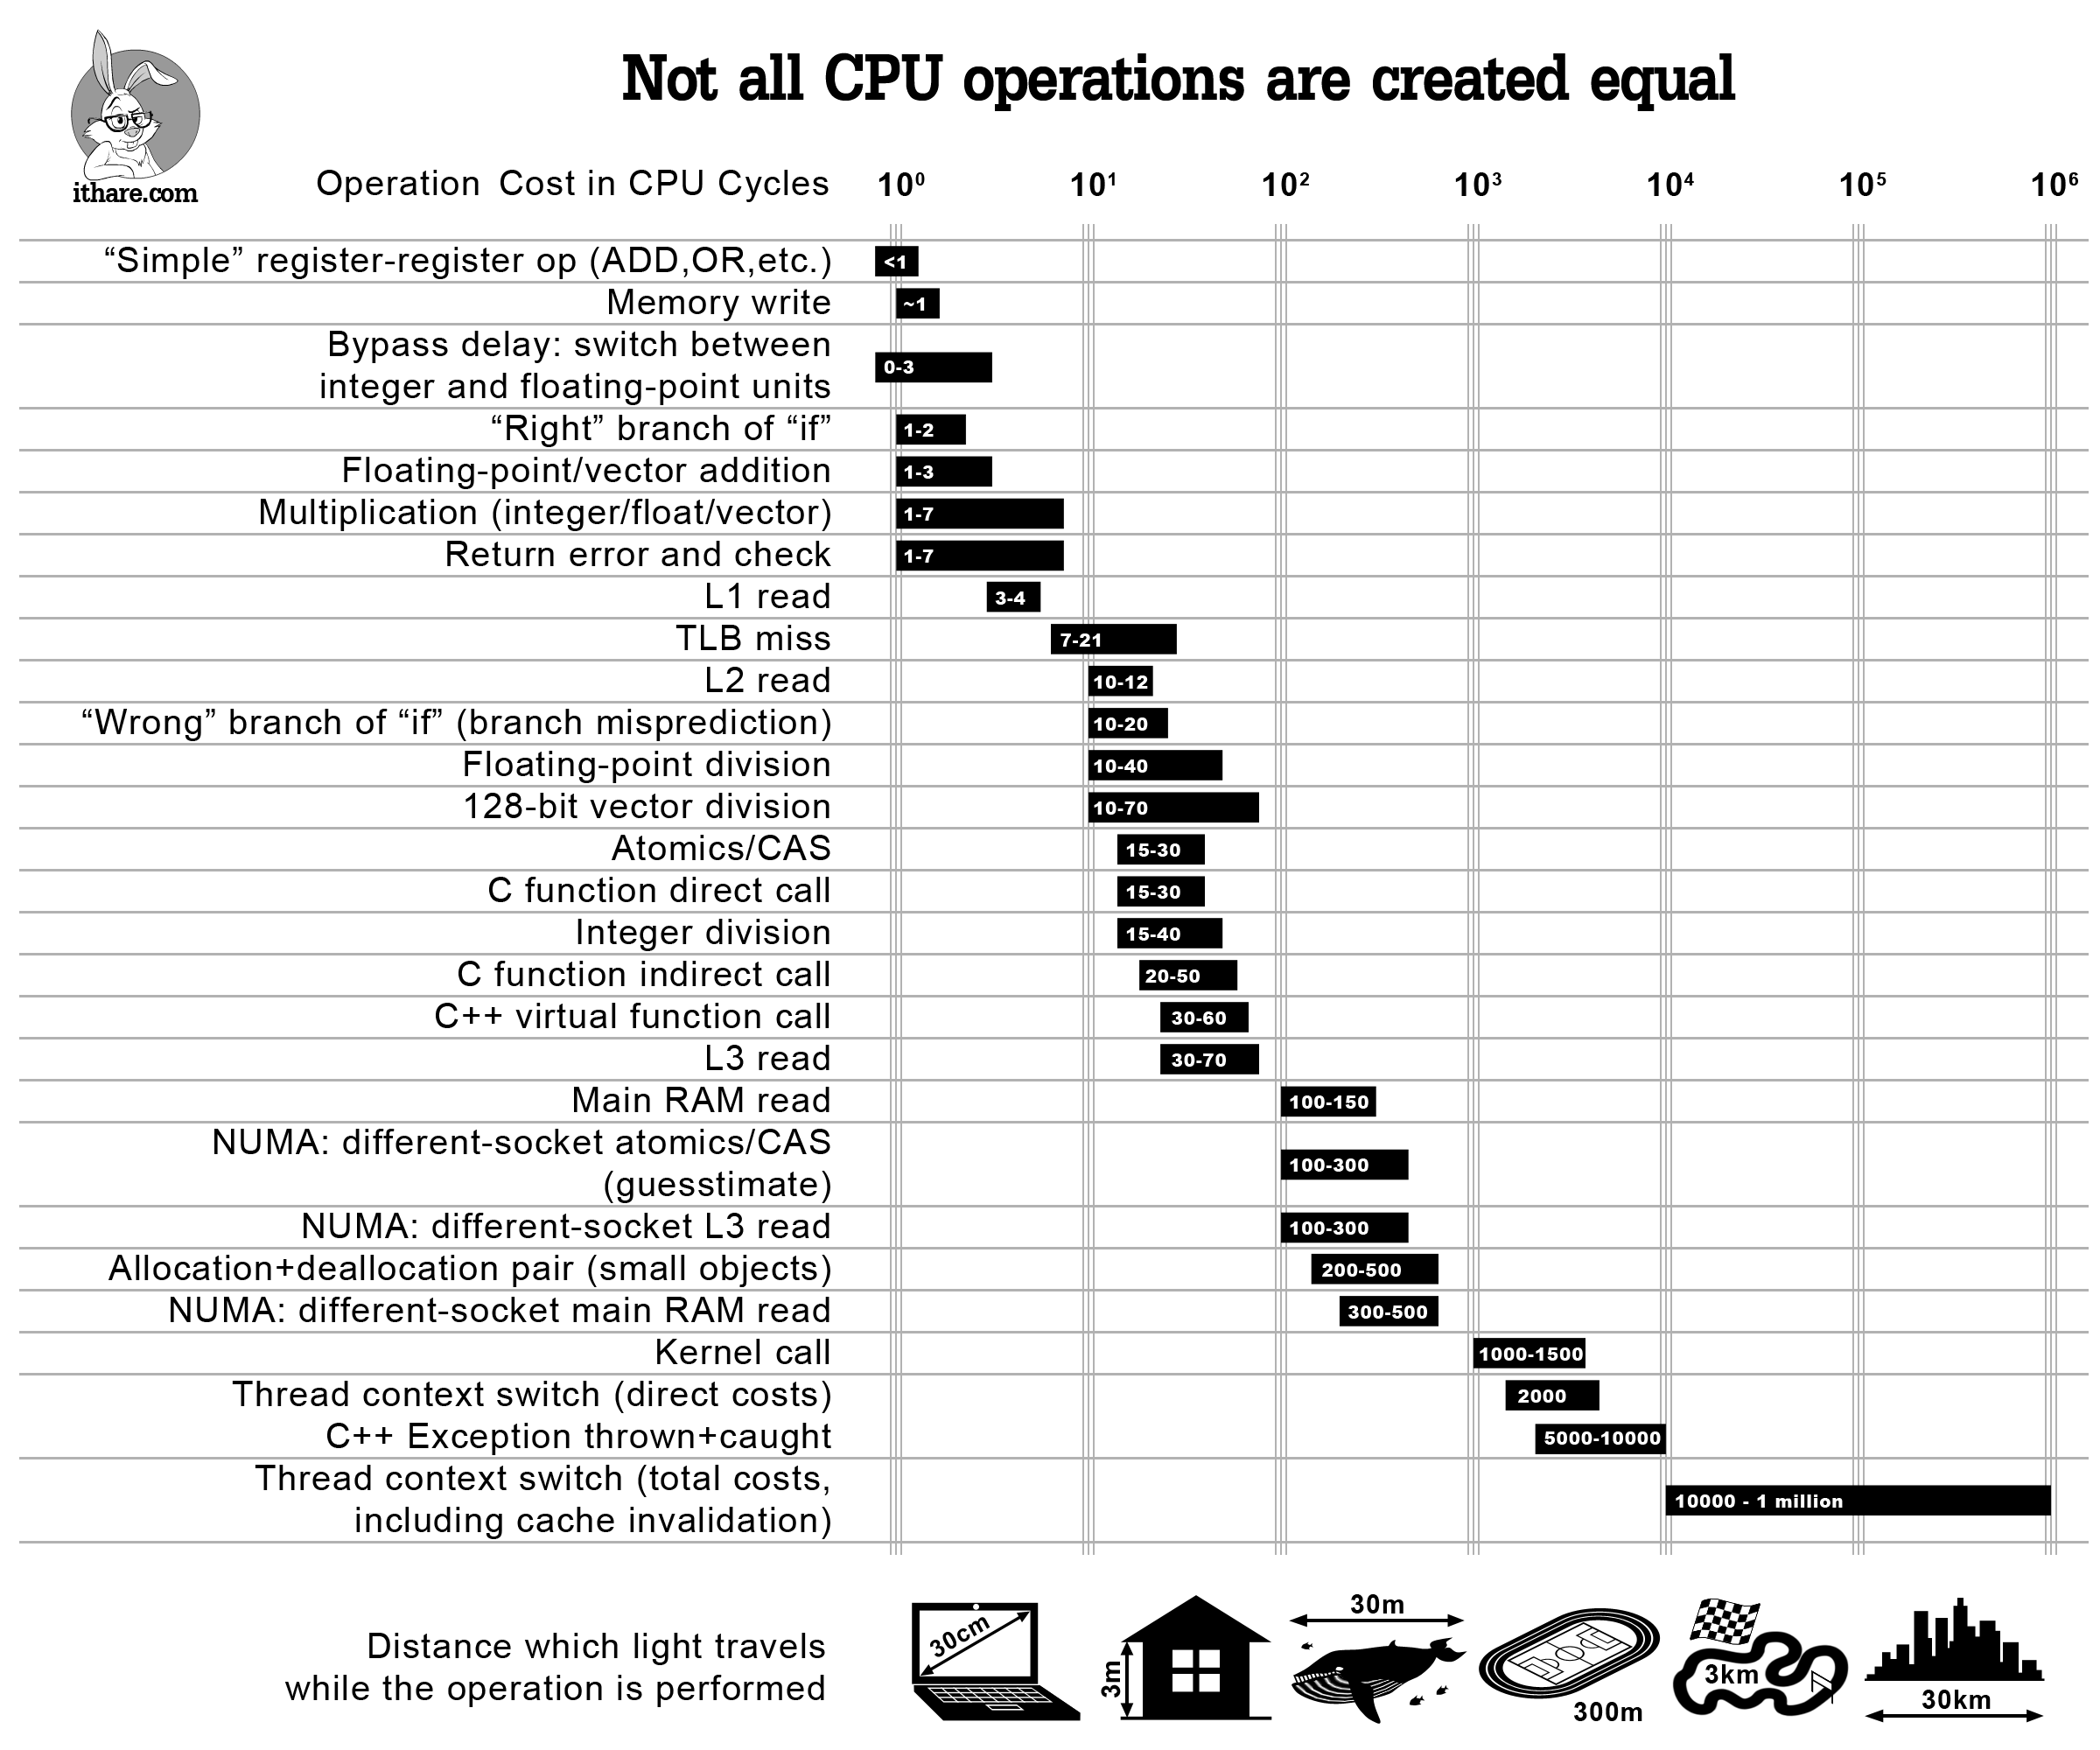
\includegraphics[width=17.25cm]{./fig/part101_infographics_v08.png}
  \caption{
    Infographics: Operation Costs in CPU Clock Cycles \citep{NoBugsHare2016}.
  }
  \label{fig_part101_infographics}
\end{figure}

%\section{セクション1}
%内容.

%\section{セクション2}
%図/表など.


\chapter*{Acknowledgments/謝辞}%
\addcontentsline{toc}{chapter}{Acknowledgments/謝辞}

感謝の気持ちを述べる.




\renewcommand{\bibname}{参考文献} % jecon.bst だと bib の doi を読み込めずエラーを吐くので,ここだけ,削除すること.
\bibliographystyle{jecon}
\nocite{*} % 文献の引用がない場合のエラーを抑制.
\bibliography{09_References}

\end{document}
